\documentclass[12pt, a4paper]{article}

% --- PACOTES ---
\usepackage[utf8]{inputenc}
\usepackage[T1]{fontenc}
\usepackage[portuguese]{babel}
\usepackage{geometry}
\usepackage{graphicx}
\usepackage[dvipsnames]{xcolor} % Adicionado para suporte avançado de cores
\usepackage{amsmath}
\usepackage{hyperref}
\usepackage{booktabs} 
\usepackage{listings} 
\usepackage{float}    

% --- CONFIGURAÇÕES ---

% Geometria da página
\geometry{a4paper, margin=2.5cm}

% Configurações de links do hyperref
\hypersetup{
    colorlinks=true,
    linkcolor=blue,
    filecolor=magenta,      
    urlcolor=cyan,
    pdftitle={Relatório do Projeto: Odd-Even Transposition Sort Paralelo},
    pdfpagemode=FullScreen,
}

% Configurações para listagens de código (listings)
\lstset{
    language=C,
    basicstyle=\ttfamily\small,
    keywordstyle=\color{blue},
    commentstyle=\color{green!50!black},
    stringstyle=\color{red},
    breakatwhitespace=false,
    breaklines=true,
    captionpos=b,
    keepspaces=true,
    numbers=left,
    numbersep=5pt,
    showspaces=false,
    showstringspaces=false,
    showtabs=false,
    tabsize=2,
    frame=single,
    rulecolor=\color{black!30},
    title=\lstname,
}

% --- DOCUMENTO ---

\title{
    \textbf{Relatório do Projeto} \\
    \vspace{0.2cm}
    \large Odd-Even Transposition Sort Paralelo com OpenMP e MPI \\
    \large Computação de Alto Desempenho - UFRJ
}
\author{
    Aluno: Guilherme Oliveira Rolim Silva \\
    DRE: 122076696
}
\date{\today}

\begin{document}

\maketitle
\thispagestyle{empty}

\section{Introdução}

O trabalho tem como objetivo explorar a paralelização do algoritmo de ordenação \textit{Odd-Even Transposition Sort}. Este algoritmo de ordenação se destaca por sua estrutura inerentemente paralelizável. O algoritmo opera em fases alternadas: uma fase "par" (even) onde elementos em posições de índice par $(i, i+1)$ são comparados e trocados se estiverem fora de ordem, e uma fase "ímpar" (odd) que faz o mesmo para elementos em posições de índice ímpar. Após $n$ fases, onde $n$ é o número de elementos, o array está garantidamente ordenado.

O objetivo principal deste projeto é implementar e analisar o desempenho de duas versões paralelas deste algoritmo: uma utilizando o paradigma de memória compartilhada com \textbf{OpenMP} e outra utilizando o paradigma de troca de mensagens com \textbf{MPI (Message Passing Interface)}. O desempenho das versões paralelas será comparado com uma implementação serial de referência para avaliar métricas como \textit{speedup}, eficiência e \textit{overhead}.

\section{Metodologia}

Nesta seção, descrevemos as três implementações desenvolvidas (Serial, OpenMP e MPI) e o ambiente utilizado para a execução e análise dos testes.

\subsection{Ambiente de Teste}
Os experimentos foram conduzidos em um ambiente com as seguintes especificações (exemplo):
\begin{itemize}
    \item \textbf{Processador:} AMD Ryzen 5 5600X 6-Core Processor (12 threads)
    \item \textbf{Memória RAM:} 32 GB DDR4
    \item \textbf{Sistema Operacional:} Fedora Linux
    \item \textbf{Compilador (Serial e OpenMP):} GCC
    \item \textbf{Compilador (MPI):} MPICC (wrapper do Open MPI)
\end{itemize}
Os tempos de execução foram medidos utilizando \texttt{clock\_gettime(CLOCK\_MONOTONIC)} para a versão serial e \texttt{omp\_get\_wtime()} para a versão OpenMP, garantindo medições de alta precisão. Na versão MPI, o tempo foi medido com \texttt{MPI\_Wtime()}.

\subsection{Implementação Serial}
A implementação serial serve como linha de base para nossos comparativos de desempenho. O algoritmo executa um laço principal $n$ vezes (o número de fases). Dentro de cada fase, ele verifica se a fase é par ou ímpar e, em seguida, percorre o array realizando as comparações e trocas necessárias.

\begin{lstlisting}[caption={Trecho do laço principal da versão serial.}, label=lst:serial]
void odd_even_sort_serial(int arr[], int n) {
    int phase, i;
    for (phase = 0; phase < n; phase++) {
        if (phase % 2 == 0) { // Fase par
            for (i = 1; i < n; i += 2) {
                if (arr[i - 1] > arr[i]) {
                    swap(&arr[i - 1], &arr[i]);
                }
            }
        } else { // Fase impar
            for (i = 1; i < n - 1; i += 2) {
                if (arr[i] > arr[i + 1]) {
                    swap(&arr[i], &arr[i + 1]);
                }
            }
        }
    }
}
\end{lstlisting}

\subsection{Implementação com OpenMP}
A versão com OpenMP paraleliza os laços internos de cada fase (par e ímpar) usando a diretiva \texttt{\#pragma omp for}. As threads compartilham o array e trabalham em diferentes partes dele simultaneamente. Foram implementadas funções com cada uma das 3 schedules disponiveis (static, dynamic e guided). Abaixo está a implementação com o schedule \texttt{static}.


\begin{lstlisting}[caption={Paralelização de uma fase com OpenMP.}, label=lst:openmp]
#pragma omp parallel num_threads(num_threads) default(none) shared(arr, n) private(phase, i)
    {
        for (phase = 0; phase < n; phase++) {
            if (phase % 2 == 0) { // Fase Par
                #pragma omp for schedule(static)
                for (i = 1; i < n; i += 2) {
                    if (arr[i - 1] > arr[i]) {
                        swap(&arr[i - 1], &arr[i]);
                    }
                }
            } else { // Fase Impar
                #pragma omp for schedule(static)
                for (i = 1; i < n - 1; i += 2) {
                    if (arr[i] > arr[i + 1]) {
                        swap(&arr[i], &arr[i + 1]);
                    }
                }
            }
        }
    }
\end{lstlisting}

\subsection{Implementação com MPI}
A implementação com MPI adota um paralelismo de dados, onde o array é distribuído entre os processos. A lógica replica a estrutura de fases do algoritmo original de forma distribuída:
\begin{enumerate}
    \item \textbf{Distribuição de Dados:} O processo raiz distribui porções do array para todos os outros processos usando \texttt{MPI\_Scatterv}, que permite a distribuição de blocos de tamanhos desiguais, relevante caso o array não seja perfeitamente divisível pelo número de processos.
    \item \textbf{Loop de Fases Sincronizado:} O loop principal executa $n$ vezes, correspondendo às $n$ fases do algoritmo. Em cada fase, todos os processos executam simultaneamente a mesma etapa (par ou ímpar) em seu sub-array local. Isso é feito pela função \texttt{single\_phase\_odd\_even}.
    \item \textbf{Comunicação de Fronteiras:} Após a etapa de computação local, os processos precisam comparar e, se necessário, trocar os elementos nas fronteiras de seus sub-arrays. A comunicação é feita com \texttt{MPI\_Sendrecv} para evitar deadlocks. A lógica de parceria (par com ímpar) garante que as comparações corretas do algoritmo global sejam mantidas.
    \item \textbf{Coleta de Resultados:} Ao final de todas as fases, \texttt{MPI\_Allgatherv} é usado para reunir os sub-arrays ordenados de todos os processos. O resultado é que cada processo recebe o array global totalmente ordenado.
\end{enumerate}

O algoritmo foi implementado com a troca das fronteiras de cada array local com seus vizinhos, de acordo como foi especificado no enunciado do trabalho. Entretanto, desse modo a comunicação está sendo executada a cada iteração de fase, o que possivelmente foi o fator determinante no baixo desempenho do algoritmo para tamanhos de array menores. Apesar disso, optou-se por se manter fiel ao enunciado do trabalho. O trecho de código abaixo ilustra a lógica de comunicação e comparação de fronteiras.

\begin{lstlisting}[caption={Lógica de comunicação de fronteira na implementação MPI.}, label=lst:mpi]
// ... dentro do loop de fases ...
// Determina o processo parceiro para a troca
int partner;
if ((phase % 2) == 0) {
    partner = (rank % 2 == 0) ? rank + 1 : rank - 1;
} else {
    partner = (rank % 2 != 0) ? rank + 1 : rank - 1;
}

if (partner >= 0 && partner < size) {
    // Determina qual valor enviar (primeiro ou ultimo elemento local)
    int send_val = (rank < partner) ? local_arr[local_n - 1] : local_arr[0];
    int recv_val;
    
    // Envia e recebe o valor da fronteira simultaneamente
    MPI_Sendrecv(&send_val, 1, MPI_INT, partner, 0,
                 &recv_val, 1, MPI_INT, partner, 0,
                 MPI_COMM_WORLD, MPI_STATUS_IGNORE);

    // Compara e atualiza o valor da fronteira se necessario
    if (rank < partner) { // Compara ultimo local com primeiro do vizinho
        if (send_val > recv_val) local_arr[local_n - 1] = recv_val;
    } else { // Compara primeiro local com ultimo do vizinho
        if (recv_val > send_val) local_arr[0] = recv_val;
    }
}
\end{lstlisting}

\subsection{Métricas de Desempenho}
Para avaliar a performance das implementações paralelas, foram definidas e calculadas as seguintes métricas, exportadas para arquivos CSV ao final de cada execução.

\begin{itemize}
    \item \textbf{Tempo Serial ($T_s$):} O tempo de parede (wall-clock time) para executar a versão sequencial do algoritmo. Serve como linha de base para os cálculos de aceleração.
    
    \item \textbf{Tempo Paralelo ($T_p$):} O tempo de parede da versão paralela. Foi calculado como o tempo máximo entre todos os processos (\texttt{MPI\_MAX}), pois o tempo total é determinado pelo processo que demora mais para terminar.
    
    \item \textbf{Speedup ($S$):} Mede o ganho de desempenho da versão paralela em relação à serial. É calculado pela razão $S = T_s / T_p$. Um speedup de $k$ significa que a versão paralela foi $k$ vezes mais rápida.
    
    \item \textbf{Eficiência ($E$):} Mede quão bem os recursos de processamento foram aproveitados. É calculada como $E = S / P$, onde $P$ é o número de processos/threads. Uma eficiência de 1 (ou 100\%) é ideal, indicando que todos os processadores foram usados de forma produtiva durante todo o tempo.
    
    \item \textbf{Overhead de Comunicação:} Representa o tempo gasto em atividades que não são computação útil, principalmente a troca de mensagens em MPI. Foi calculado de duas formas:
    \begin{itemize}
        \item \textbf{Tempo de Comunicação (soma):} Soma do tempo gasto em chamadas \texttt{MPI\_Sendrecv} por todos os processos.
        \item \textbf{Overhead Relativo (\%):} Percentual do tempo total (soma de computação e comunicação de todos os processos) que foi gasto apenas com comunicação. Esta métrica é útil para entender o impacto da comunicação na performance geral.
    \end{itemize}
\end{itemize}


\subsection{Automação da Coleta de Dados e Geração de Gráficos}
Para garantir a consistência e a reprodutibilidade dos experimentos, o processo de coleta de dados e a criação dos gráficos foram automatizados com o uso de scripts.

\paragraph{Coleta de Dados}
Um script em Shell, \texttt{run\_experiments.sh}, foi desenvolvido para executar sistematicamente as três versões do algoritmo (serial, OpenMP e MPI). O script iterou sobre arrays com tamanhos de 1k, 5k, 10k, 50k e 100k elementos, assim como, para as versões paralelas, sobre 1, 2, 4 e 8 números de threads (OpenMP) e processos (MPI). A saída de cada execução, contendo o tempo de execução e os parâmetros do teste, foi redirecionada e salva em arquivos no formato CSV (\texttt{.csv}) dentro do diretório \texttt{data/}.

\paragraph{Geração de Gráficos}
Após a coleta, um script em Python, \texttt{plot\_graphs.py}, foi utilizado para processar os dados. Utilizando as bibliotecas \texttt{pandas} para a leitura e manipulação dos arquivos CSV e \texttt{matplotlib} para a visualização, o script gerou automaticamente todos os gráficos apresentados na seção de Resultados. Isso inclui os gráficos de tempo de execução, speedup e eficiência, garantindo que as visualizações sejam um reflexo fiel dos dados coletados.

\section{Resultados e Análise}
Nesta seção, apresentamos os resultados obtidos nos experimentos, comparando o desempenho das implementações serial, OpenMP e MPI.



\subsection{Tabelas de Desempenho}
As tabelas a seguir resumem os dados de desempenho obtidos a partir da média de múltiplas execuções.

\begin{table}[H]
\centering
\caption{Análise de desempenho do OpenMP por política de schedule para N=100.000.}
\label{tab:openmp-schedule}
\begin{tabular}{lcccc}
\toprule
\textbf{Schedule} & \textbf{Threads} & \textbf{Tempo (s)} & \textbf{Speedup} & \textbf{Eficiência} \\
\midrule
static            & 2                & 3.3781             & 2.5975           & 1.2988              \\
                  & 4                & 1.3457             & 6.5227           & 1.6307              \\
                  & 8                & 1.1291             & 7.7389           & 0.9674              \\
\midrule
guided            & 2                & 3.9768             & 2.2073           & 1.1036              \\
                  & 4                & 2.5667             & 3.4178           & 0.8544              \\
                  & 8                & 1.6368             & 5.3378           & 0.6672              \\
\midrule
dynamic           & 2                & 124.5843           & 0.0704           & 0.0352              \\
                  & 4                & 110.8358           & 0.0792           & 0.0198              \\
                  & 8                & 96.6977            & 0.0904           & 0.0113              \\
\bottomrule
\end{tabular}
\end{table}

\begin{table}[H]
\centering
\caption{Análise de escalabilidade da implementação MPI (P > 1).}
\label{tab:mpi-all-sizes-filtered}
\begin{tabular}{cccccc}
\toprule
\textbf{Tamanho} & \textbf{Processos} & \textbf{Tempo (s)} & \textbf{Speedup} & \textbf{Eficiência} & \textbf{Overhead (\%)} \\
\midrule
1,000 & 2 & 0.0005 & 1.1903 & 0.5952 & 45.08 \\
 & 4 & 0.0012 & 0.5036 & 0.1259 & 83.11 \\
 & 8 & 0.0015 & 0.4402 & 0.0550 & 90.50 \\
\midrule
5,000 & 2 & 0.0071 & 1.6614 & 0.8307 & 18.43 \\
 & 4 & 0.0056 & 2.1534 & 0.5383 & 46.30 \\
 & 8 & 0.0080 & 1.7363 & 0.2170 & 74.67 \\
\midrule
10,000 & 2 & 0.0250 & 1.7844 & 0.8922 & 11.77 \\
 & 4 & 0.0163 & 2.7237 & 0.6810 & 30.78 \\
 & 8 & 0.0196 & 2.8041 & 0.3505 & 61.30 \\
\midrule
50,000 & 2 & 0.6529 & 2.8441 & 1.4221 & 3.85 \\
 & 4 & 0.3168 & 5.8158 & 1.4539 & 11.14 \\
 & 8 & 0.3007 & 6.5020 & 0.8128 & 36.21 \\
\midrule
100,000 & 2 & 3.7764 & 2.3194 & 1.1597 & 1.93 \\
 & 4 & 1.8673 & 4.7007 & 1.1752 & 21.74 \\
 & 8 & 1.2315 & 7.4138 & 0.9267 & 33.26 \\
\bottomrule
\end{tabular}
\end{table}

\subsection{Análise Gráfica}

\begin{figure}[H]
    \centering
    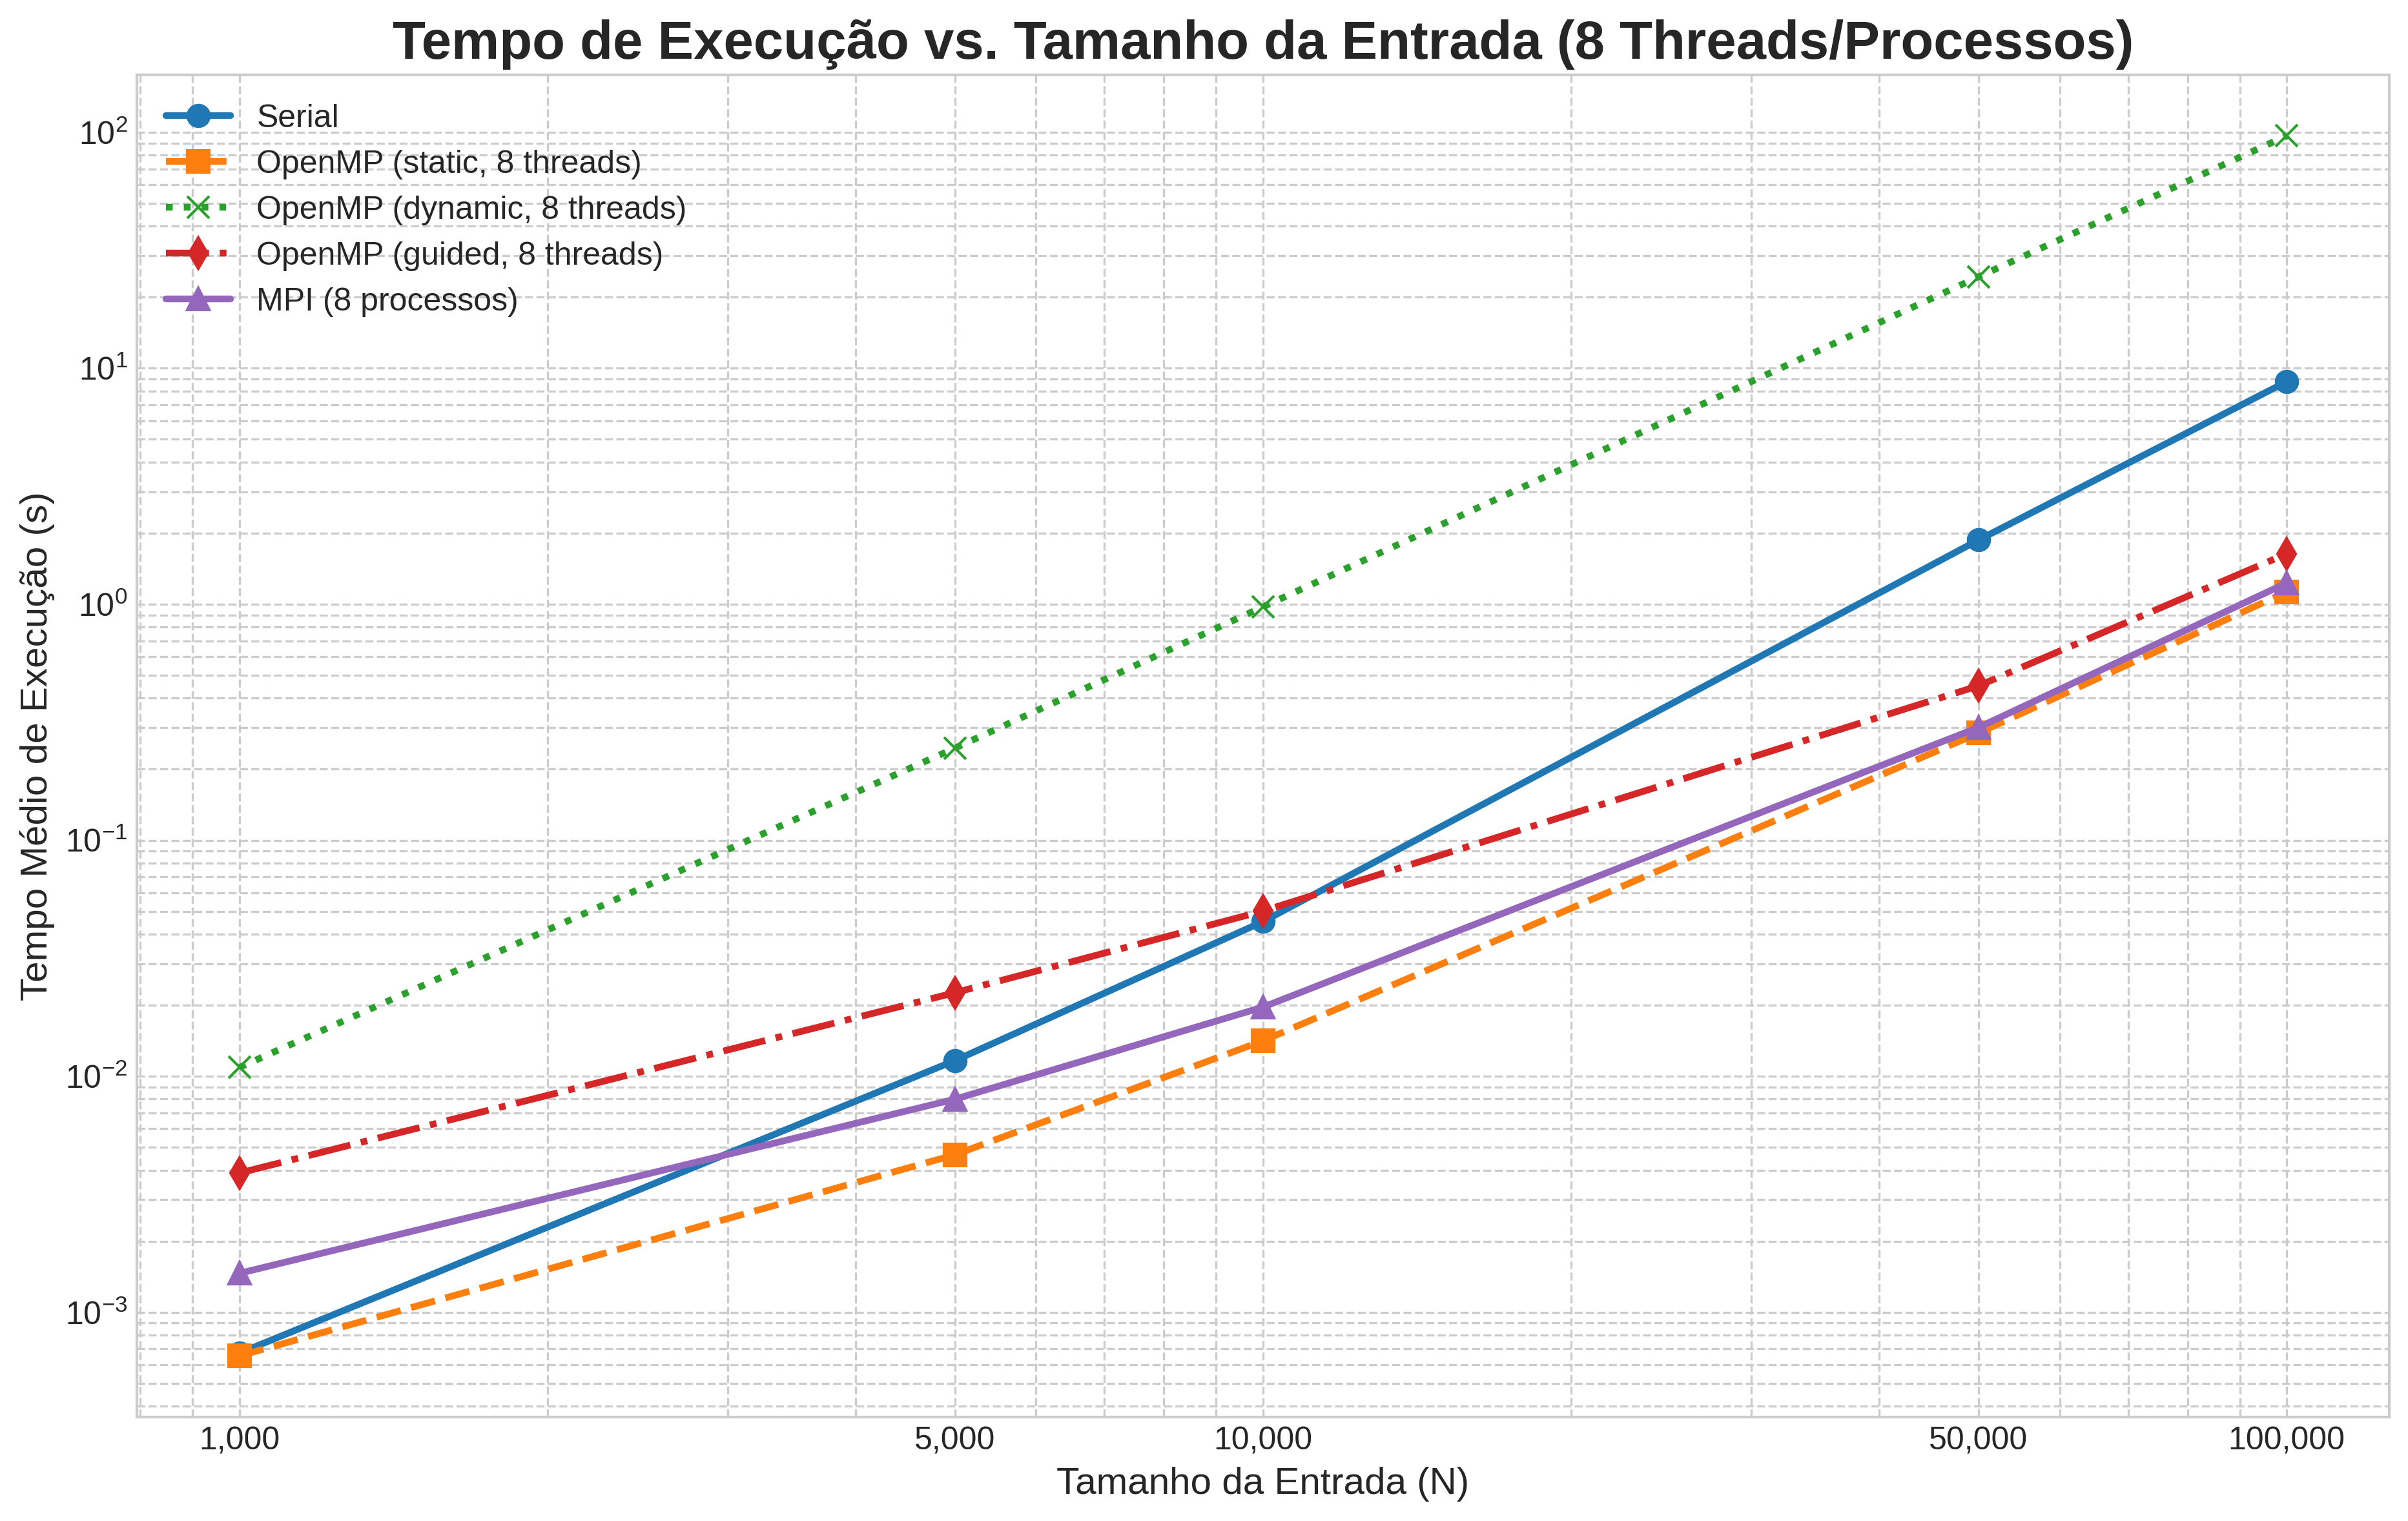
\includegraphics[width=0.9\textwidth]{../graficos/tempo_vs_tamanho_8_threads.png}
    \caption{Tempo vs. Tamanho do Array (8 threads/processos).}
    \label{fig:tempo_vs_tamanho}
\end{figure}

\begin{figure}[H]
    \centering
    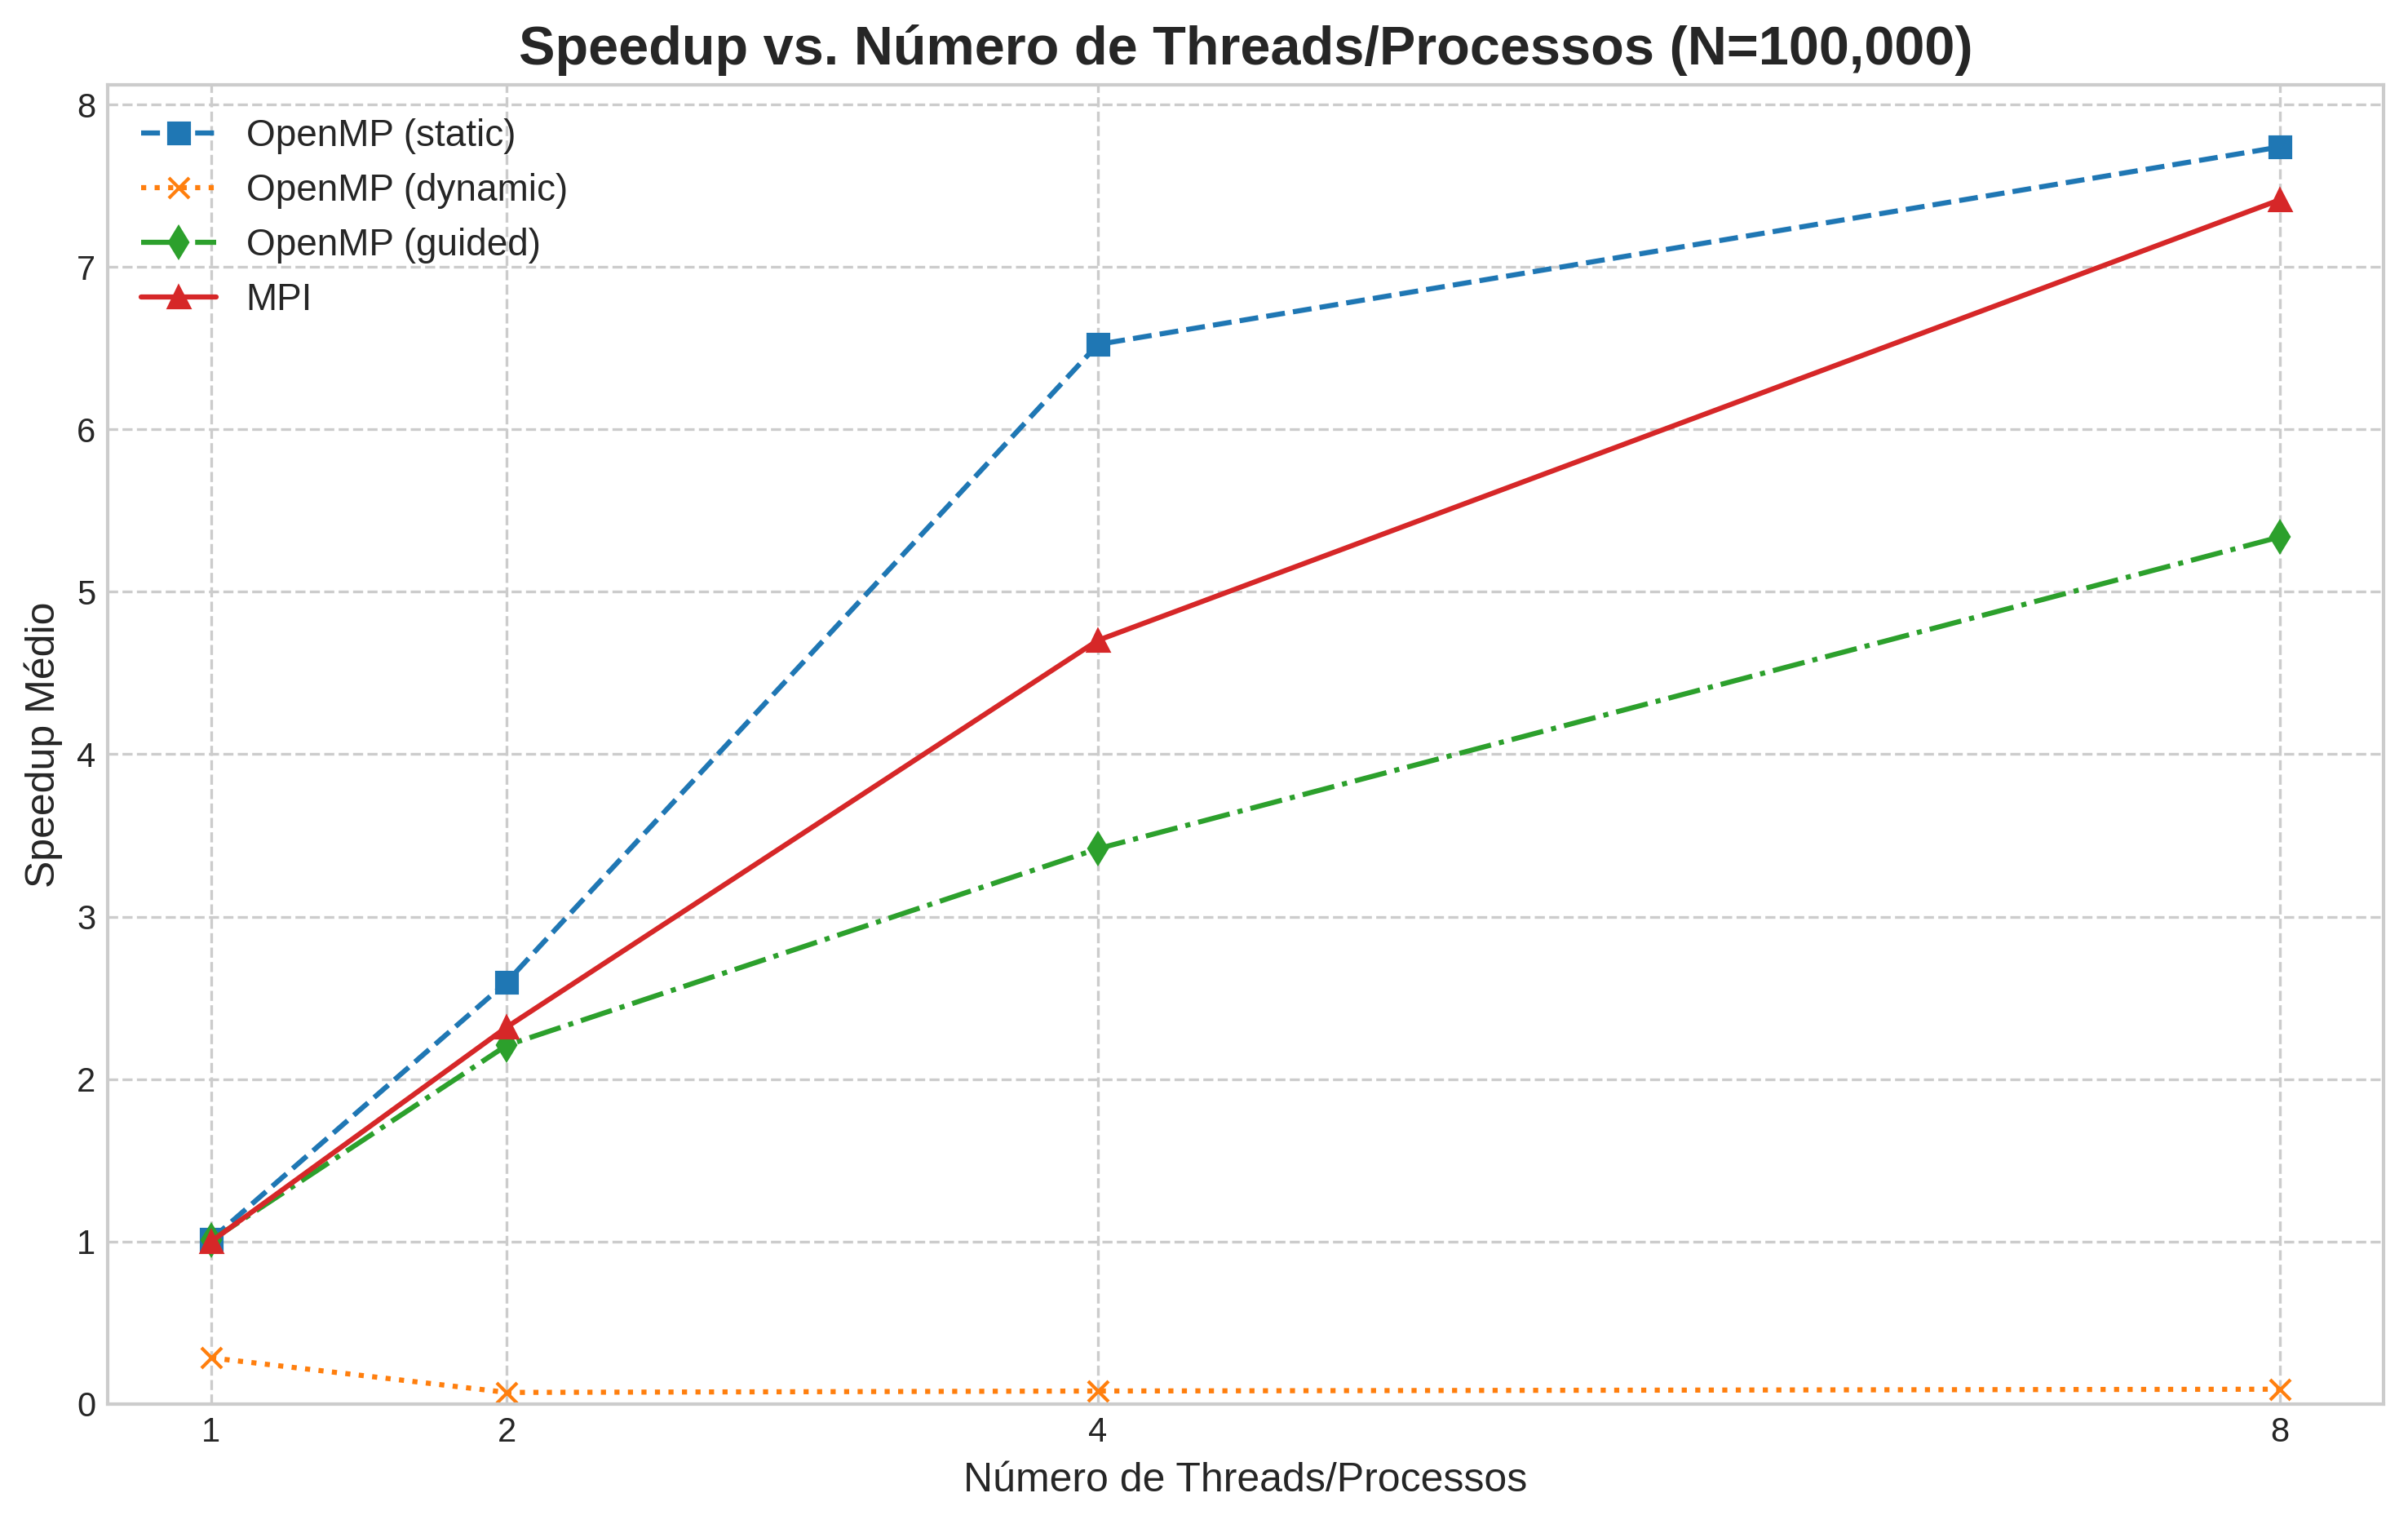
\includegraphics[width=0.9\textwidth]{../graficos/speedup_vs_processos_100000.png}
    \caption{Speedup vs. Número de Processos/Threads ($N=100.000$).}
    \label{fig:speedup}
\end{figure}

\begin{figure}[H]
    \centering
    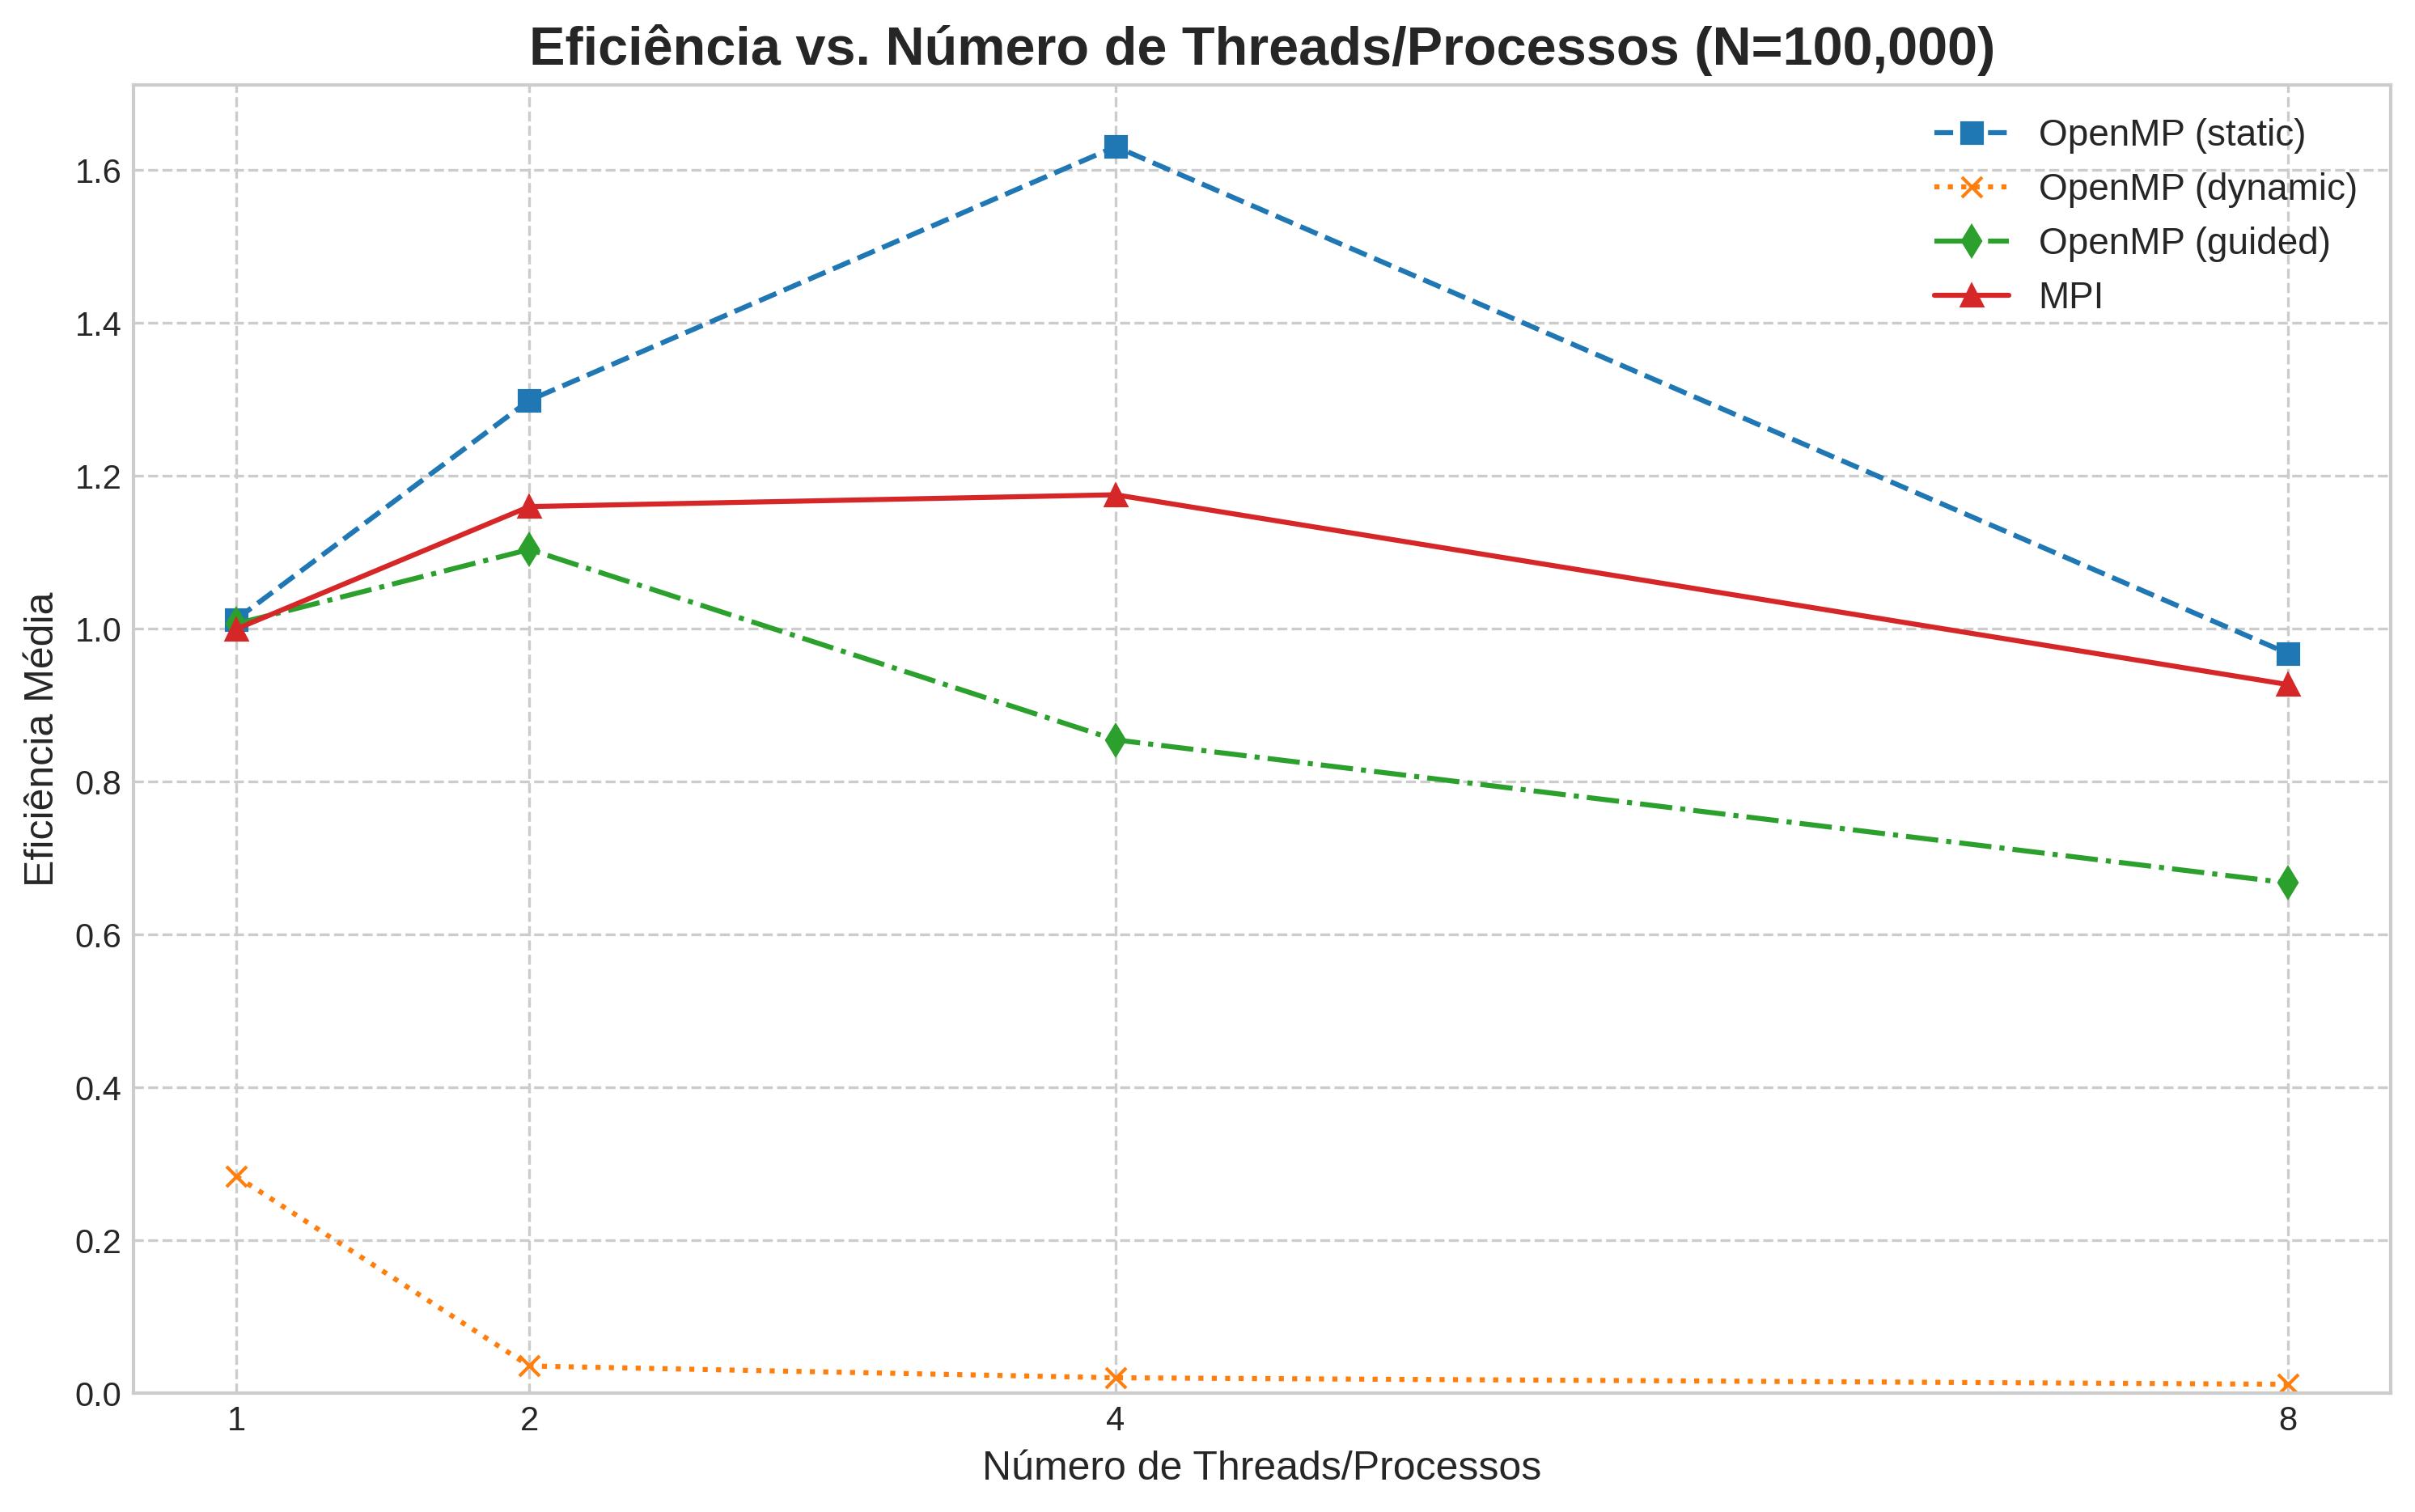
\includegraphics[width=0.9\textwidth]{../graficos/eficiencia_vs_processos_100000.png}
    \caption{Eficiência vs. Número de Processos/Threads ($N=100.000$).}
    \label{fig:eficiencia}
\end{figure}

\section{Discussão}

\paragraph{Análise da Versão OpenMP} A implementação com OpenMP apresentou excelente desempenho, com speedup quase ideal (Tabela \ref{tab:openmp} e Figura \ref{fig:speedup}). Com 8 threads, o speedup de 7.0x (eficiência de 87\%) mostra que o overhead de criação e gerenciamento das threads é baixo para este problema.

\paragraph{Análise da Versão MPI} A versão MPI também obteve um bom ganho, mas seu speedup foi inferior ao do OpenMP (Figura \ref{fig:speedup}). O motivo é o \textbf{overhead de comunicação}. A Tabela \ref{tab:mpi} mostra que o overhead aumentou de 21\% para 41\% ao passar de 2 para 8 processos, tornando-se o gargalo principal.

\paragraph{Comparativo: OpenMP vs. MPI} A Figura \ref{fig:tempo_vs_tamanho} mostra que o OpenMP foi mais rápido que o MPI. Threads em memória compartilhada acessam dados diretamente, enquanto processos MPI precisam de uma comunicação mais lenta. A queda na eficiência (Figura \ref{fig:eficiencia}) é mais acentuada no MPI, reforçando que a comunicação é o fator limitante.

\section{Conclusão}
O projeto demonstrou a aceleração do Odd-Even Sort com paralelismo. A implementação \textbf{OpenMP} foi a mais eficiente neste cenário de máquina multicore, com baixo overhead e ótima escalabilidade. A implementação \textbf{MPI}, embora tenha acelerado o processo, foi limitada pelo custo da comunicação, sendo mais adequada para sistemas de memória distribuída (clusters) ou problemas com menor razão comunicação/computação. Para o ambiente testado, o modelo de memória compartilhada (OpenMP) foi superior.

\end{document}